%
%   Prof. Dr. Julian Reichwald
%   auf Basis einer Vorlage von Prof. Dr. Jörg Baumgart
%   DHBW Mannheim
%
%
%	ACHTUNG: Für das Erstellen des Literaturverzeichnisses wird das modernere Paket biblatex
%			 in Kombination mit biber verwendet -- nicht mehr das ältere BibTex!
% 			 Bitte stellen Sie ggf. Ihre TeX-Umgebung
% 			 entsprechend ein (z.B. TeXStudio: Einstellungen --> Erzeugen --> Standard Bibliographieprogramm: biber)
%

\documentclass[
	12pt,
	BCOR=5mm,
	DIV=12,
	headinclude=on,
	footinclude=off,
	parskip=half,
	bibliography=totoc,
	listof=entryprefix,
	toc=listof,
	pointlessnumbers,
	plainfootsepline]{scrreprt}

%	Konfigurationsdatei einziehen
%		LANGUAGE SETTINGS AND FONT ENCODING 
%
%\usepackage[ngerman]{babel} 	% German language
\usepackage[utf8]{inputenc}
%\usepackage[german=quotes]{csquotes} 	% correct quotes using \enquote{}
\usepackage[T1]{fontenc}


\usepackage[english]{babel}   % For english language
\usepackage{csquotes} 	% Richtiges Setzen der Anführungszeichen mit \enquote{}

% 		HYPERREF
%
\usepackage[
hidelinks=true % keine roten Markierungen bei Links
]{hyperref}

% Zwei eigene Befehle zum Setzen von Autor und Titel. Ausserdem werden die PDF-Informationen richtig gesetzt.
\newcommand{\TitelDerArbeit}[1]{\def\DerTitelDerArbeit{#1}\hypersetup{pdftitle={#1}}}
\newcommand{\AutorDerArbeit}[1]{\def\DerAutorDerArbeit{#1}\hypersetup{pdfauthor={#1}}}
\newcommand{\Firma}[1]{\def\DerNameDerFirma{#1}}
\newcommand{\Kurs}[1]{\def\DieKursbezeichnung{#1}}


% Correct superscripts 
\usepackage{fnpct}




%		CALCULATIONS
%
\usepackage{calc} % Used for extra space below footsepline
\usepackage{amsmath}
\usepackage{amssymb}
\usepackage{mathtools}


%		BIBLIOGRAPHY SETTINGS
%

% Uncomment the next three lines for author-year-style with footnotes (Chicago)
\usepackage[backend=biber, autocite=footnote, style=authoryear, dashed=false]{biblatex} 	%Use Author-Year-Cites with footnotes
\AdaptNoteOpt\footcite\multfootcite   %will add  separators if footcite is called multiple consecutive times 
\AdaptNoteOpt\autocite\multautocite % will add  separators if autocite is called multiple consecutive times

% Uncomment the next line for IEEE-style 
% \usepackage[backend=biber, autocite=inline, style=ieee]{biblatex} 	% Use IEEE-Style (e.g. [1])

% Uncomment the next line for alphabetic style 
% \usepackage[backend=biber, autocite=inline, style=alphabetic]{biblatex} 	% Use alphabetic style (e.g. [TGK12])

% Uncomment the next two lines vor Harvard-Style 
%\usepackage[backend=biber, style=apa]{biblatex} 	
%\DeclareLanguageMapping{german}{german-apa}


\DefineBibliographyStrings{ngerman}{  %Change u.a. to et al. (german only!)
	andothers = {{et\,al\adddot}},
}

%%% Uncomment the following lines to support hard URL breaks in bibliography 
%\apptocmd{\UrlBreaks}{\do\f\do\m}{}{}
%\setcounter{biburllcpenalty}{9000}% Kleinbuchstaben
%\setcounter{biburlucpenalty}{9000}% Großbuchstaben


\setlength{\bibparsep}{\parskip}		%add some space between biblatex entries in the bibliography
\addbibresource{bibliography.bib}	%Add file bibliography.bib as biblatex resource


%		FOOTNOTES 
%
% Count footnotes over chapters
\usepackage{chngcntr}
\counterwithout{footnote}{chapter}

%	ACRONYMS
%%%
%%% WICHTIG: Installieren Sie das neueste Acronyms-Paket!!!
%%%
\makeatletter
\usepackage[printonlyused]{acronym}
\@ifpackagelater{acronym}{2015/03/20}
{%
	\renewcommand*{\aclabelfont}[1]{\textbf{\textsf{\acsfont{#1}}}}
}%
{%
}%
\makeatother

%		LISTINGS
\usepackage{listings}	%Format Listings properly
\lstset{numbers=left,
	numberstyle=\tiny,
	captionpos=b,
	basicstyle=\ttfamily\small}


%		EXTRA PACKAGES
\usepackage{graphicx} % use various graphics formats
\usepackage[german]{varioref} 	% nicer references \vref
\usepackage{caption}	%better Captions
\usepackage{booktabs} %nicer Tabs
\usepackage{array}
\usepackage{tikz}
\usetikzlibrary{shapes,matrix,positioning, arrows.meta, fit}
\usepackage{pgfplots}
\usepackage{csvsimple}
\usepackage{xltabular}

%\newcolumntype{P}[1]{>{\raggedright\arraybackslash}p{#1}}


%		ALGORITHMS
\usepackage{algorithm}
\usepackage{algpseudocode}
\renewcommand{\listalgorithmname}{Algorithmenverzeichnis }
\floatname{algorithm}{Algorithmus}


%		FONT SELECTION: Entweder Latin Modern oder Times / Helvetica
\usepackage{lmodern} %Latin modern font
%\usepackage{mathptmx}  %Helvetica / Times New Roman fonts (2 lines)
%\usepackage[scaled=.92]{helvet} %Helvetica / Times New Roman fonts (2 lines)

%		PAGE HEADER / FOOTER
%	    Warning: There are some redefinitions throughout the master.tex-file!  DON'T CHANGE THESE REDEFINITIONS!
\RequirePackage[automark,headsepline,footsepline]{scrpage2}
\pagestyle{scrheadings}
\renewcommand*{\pnumfont}{\upshape\sffamily}
\renewcommand*{\headfont}{\upshape\sffamily}
\renewcommand*{\footfont}{\upshape\sffamily}
\renewcommand{\chaptermarkformat}{}
\RedeclareSectionCommand[beforeskip=0pt]{chapter}
\clearscrheadfoot

\ifoot[\rule{0pt}{\ht\strutbox+\dp\strutbox}DHBW Mannheim]{\rule{0pt}{\ht\strutbox+\dp\strutbox}DHBW Mannheim}
\ofoot[\rule{0pt}{\ht\strutbox+\dp\strutbox}\pagemark]{\rule{0pt}{\ht\strutbox+\dp\strutbox}\pagemark}

\ohead{\headmark}

\begin{document}

%% BITTE GEBEN SIE HIER DEN TITEL UND DIE AUTORIN / DEN AUTOR DER ARBEIT AN!
%% DIESE INFORMATIONEN _MÜSSEN_ GESETZT SEIN, UM TITELBLATT, ABSTRACT UND
%% EIGENSTÄNDIGKEITSERKLÄRUNG AUTOMATISCH ANZUPASSEN!
\TitelDerArbeit{Konzeptionelle Entwicklung eines Lokalisierungstools für Movelets}
\AutorDerArbeit{Fabian Wolf}
\Firma{Honeywell International Inc.}
\Kurs{WWI17SEC}

\begin{titlepage}
\begin{minipage}{\textwidth}
		\vspace{-2cm}
		\noindent 
\includegraphics{img/firmenlogo.pdf} \hfill   
\includegraphics{img/dhbwlogo.pdf}
\end{minipage}
\vspace{1em}
\sffamily
\begin{center}
	\textsf{\large{}Duale Hochschule Baden-W\"urttemberg\\[1.5mm] Mannheim}\\[2em]
	\textsf{\textbf{\Large{}Projektarbeit 1}}\\[3mm]
	\textsf{\textbf{\DerTitelDerArbeit}} \\[1.5cm]
	\textsf{\textbf{\Large{}Studiengang Wirtschaftsinformatik}\\[3mm] \textsf{Studienrichtung Software Engineering}}
	
	\vspace{3em}
\vfill

\begin{minipage}{\textwidth}

\begin{tabbing}
	Wissenschaftlicher Betreuer: \hspace{0.85cm}\=\kill
	Verfasser: \> \DerAutorDerArbeit \\[1.5mm]
	Matrikelnummer: \> 7345461 \\[1.5mm]
	Firma: \> \DerNameDerFirma  \\[1.5mm]
	Abteilung: \> Research \& Development \\[1.5mm]
	Kurs: \> \DieKursbezeichnung \\[1.5mm]
	Studiengangsleiter: \> Prof. Dr.-Ing. habil. Dennis Pfisterer  \\[1.5mm]
	Wissenschaftlicher Betreuer: \>Prof. Dr.-Ing. habil. Dennis Pfisterer \\
	\> dennis.pfisterer@dhbw-mannheim.de \\
	\> +49 62 14105-1253 \\[1.5mm]
	Firmenbetreuer: \> Herr Oliver Erlenkaemper \\
	\> Oliver.Erlenkaemper@Honeywell.com \\
	\> +49 62 18545-0237 \\[1.5mm]
	Bearbeitungszeitraum: \> 07.08.2018 -- \today
\end{tabbing}
\end{minipage}

\end{center}

\end{titlepage}

\pagenumbering{roman} % Römische Seitennummerierung
\normalfont

%--------------------------------
% Start der Vortexte der Arbeit
%--------------------------------

%	Kurzfassung
\chapter*{Kurzfassung}
%\begingroup
%\begin{table}[h!]
%\setlength\tabcolsep{0pt}
%\begin{tabular}{p{3.7cm}p{11.7cm}}
%Titel & \DerTitelDerArbeit \\
%Verfasser/in: & \DerAutorDerArbeit \\
%Kurs: & \DieKursbezeichnung \\
%Ausbildungsstätte: & \DerNameDerFirma\\
%\end{tabular}
%\end{table}
%\endgroup
%Einführung und Motivation
Softwareprodukte werden heutzutage weltweit vermarktet. Infolgedessen müssen Unternehmen ihre Softwareprodukte effizient lokalisieren, falls sie sich erfolgreich auf dem Weltmarkt behaupten wollen. 
\autocite[Vgl.][S. 1]{Schmitz.2000}
\autocite[Vgl.][S. 1]{Reineke.2005} 
Aus diesem Grund ist Software zur Automatisierung der Lokalisierung nötig. 
%Forschungslücke
Derzeit wird von Movilizer keine Software zur Lokalisierung von Movelets eingesetzt. 
%Ziel
Ziel dieser Arbeit ist die Konzeption einer Software, welche zu übersetzende und übersetzte Strings der Texte eines Movelets automatisiert verarbeitet. Diese Software wird im Folgenden als Lokalisierungstool bezeichnet. 
%Methode
Anhand von Literaturrecherche werden verschiedene Konzepte analysiert und diskutiert. 
%Ergebnisse
Das resultierende Lokalisierungstool extrahiert zu übersetzende Strings in XLIFF Dateien anhand von ITS und einer $\_()$ Auszeichnung. Die extrahierten Strings erhalten eine Übersetzung, welche von dem Lokalisierungstool genutzt wird um die ausgezeichneten Strings zu ersetzen. 
%Interpretation
Resultierend daraus ist dieses Lokalisierungstool der Anfang der Automatisierung der Lokalisierung von Movelets.

%	Inhaltsverzeichnis
\tableofcontents

%	Abbildungsverzeichnis
\listoffigures

%	Listingsverzeichnis
 \lstlistoflistings

% 	Abkürzungsverzeichnis (siehe Datei acronyms.tex!)
\clearpage
\chapter*{Abkürzungsverzeichnis}	
\addcontentsline{toc}{chapter}{Abkürzungsverzeichnis}


\begin{acronym}[RDBMS]
	\acro{MEL}{Movilizer Expression Language}
	\acro{MXML}{Movilizer Extensible Markup Language}
	\acro{XML}{Extensible Markup Language}
	\acro{NVDL}{Namespace-based Validation Dispatching Language}
	\acro{XPATH}{XML Path Language}
	\acro{.po}{Portable Object}
	\acro{.mo}{Machine Object}
	
	\acro{TMX}{Translation Memory Exchange}
	\acro{XML:TM}{XML Text Memory}
	\acro{XLIFF}{ XML Localisation Interchange File Format}
	\acro{SRX}{Segmentation Rules Exchange}
	\acro{GMX-V}{Global Information Management Metrics Volume}
	\acro{UTX}{Universal Terminology Exchange}
	\acro{TBX}{Term Base Exchange}
	\acro{OLIF}{Open Lexicon Interchange Format}
	\acro{Trans-WS}{Translation Web Services}
	\acro{ITS}{Internationalization Tag Set}
	
	
	\acro{GALA}{Globalization and Localization Association}
	\acro{LISA}{Localization Industry Standards Association}
	\acro{OASIS}{Organization for the Advancement of Structured Information Standards}
	\acro{AAMT}{Asia-Pacific Association for Machine Translation}
	\acro{W3C}{World Wide Web Consortium}
	
	\acro{NLP}{Natural Language Processing}
	\acro{CAT}{Computer Assisted Translation}
	\acro{TM}{Translation Memory}
\end{acronym}


%--------------------------------
% Start des Textteils der Arbeit
%--------------------------------
\clearpage
\ihead{\chaptername~\thechapter} % Neue Header-Definition (inner header)
\ohead{\headmark} % Neue Header-Definition (outer header)
\pagenumbering{arabic}  % Arabische Seitenzahlen

\chapter{Einleitung}
\section{Allgemeine Themenrelevanz}
Softwareprodukte werden heutzutage weltweit vermarktet. In der Konsequenz müssen Unternehmen ihre Softwareprodukte an die Anforderungen verschiedener regionaler Märkte anpassen, falls sie sich erfolgreich auf dem Weltmarkt behaupten wollen. Aufgrund dieser Entwicklung zählt Lokalisierung heute zu den Schlüsselbegriffen einer globalen Marktwirtschaft. 
\autocite[Vgl.][S. 1]{Schmitz.2000}
\autocite[Vgl.][S. 1]{Reineke.2005} 
Lokalisierung alleine reicht jedoch nicht, um sich gegen Konkurrenten durchzusetzen. Faktoren wie Qualität, Dauer und Kosten sind von großer Bedeutung. Daher ist die Automatisierung von Unterprozessen der Lokalisierung  durch Software erforderlich. 
\autocite[Vgl.][S. 1]{Zydron.2009}
Derzeit wird von Movilizer keine Software zur Lokalisierung von Movelets eingesetzt. 
\section{Ziel dieser Projektarbeit}
Ziel dieser Arbeit ist die Konzeption einer Software, welche zu übersetzende und übersetzte Strings der Texte eines Movelets automatisiert verarbeitet. Resultierend daraus verringert die Software den Aufwand des Prozesses der Lokalisierung. Aufgrund dessen, dass die Software einen Unterprozess der Lokalisierung automatisiert, wird sie im Folgenden als Lokalisierungstool bezeichnet. 
\par
Weitere Unterprozesse der Lokalisierung werden von diesem Lokalisierungstool nicht umgesetzt. Hierzu zählen:
\begin{itemize}
	\item Übersetzung
	\item Verwendung geeigneter Zeichensätze
	\item Übersetzung verknüpfter Strings
	\item Anpassung von Grafiken und Symbolen
	\item Anpassen der Benutzeroberfläche an Textlängen und Flussrichtungen
	\item Anpassung an geltendes Recht
	\item Anpassung der Formate für Adresse, Datum et cetera
	\item Anpassung der Maßeinheiten für Gewicht, Währung, et cetera
	\item Anpassung der Sortierung und Suche
\end{itemize}
\autocite[Vgl.][S. 423]{HassellCorbiell.2001}
\autocite[Vgl.][]{Asnes.2010}
\autocite[Vgl.][]{Wagner.2017}
\par
Im Verlauf dieser Arbeit werden zunächst die sich aus dem Ziel ergebenden Anforderungen formuliert. Des Weiteren, werden die möglichen Lösungsansätze zu den einzelnen Anforderungen formuliert und unter Berücksichtigung vorausgegangener Erkenntnisse diskutiert. Die Lösungsansätze ergeben sich anhand von Literaturrecherche. Sollten sich aus der Diskussion neue Anforderungen ergeben, wird dieses Verfahren iterativ angewandt. Aus der Gesamtheit aller erarbeiteten Lösungen ergibt sich das Konzept des Lokalisierungstools. 
\chapter{Begriffe}
\section{Globalisierung}
Als Globalisierung bezeichnet man alle Aktivitäten eines Unternehmens mit dem Ziel der Vermarktung eines (Software-)Produkts außerhalb des nationalen, lokalen Marktes. Zu diesem Zweck sind technische, wirtschaftliche und gesetzliche Aspekte des Zielmarktes besonders zu berücksichtigen. Infolgedessen ist die Globalisierung im Kontext der betriebswirtschaftlichen und kaufmännischen Unternehmensführung zu betrachten.
\autocite[Vgl.][S. 1]{Reineke.2005}
\autocite[Vgl.][ S. 2]{Schmitz.2000}
\section{Internationalisierung}
\label{sec:internationalisierung}
Als Internationalisierung bezeichnet man die Entwicklung von (Software-)Produkten auf eine Weise, die eine möglichst schnelle Lokalisierung mit geringen Aufwand ermöglicht. Zu diesem Zweck muss das (Software-)Produkt mit einer Funktionalität entwickelt werden, die eine Anpassung an technische Konventionen, kulturelle Eigenheiten und Sprache des Zielmarktes ermöglichen. Infolgedessen ist die Internationalisierung immer im Kontext der Entwicklung zu betrachten.
\autocite[Vgl.][S. 2]{Reineke.2005}
\autocite[Vgl.][ S. 2]{Schmitz.2000}
\section{Lokalisierung}
\label{sec:lokalisierung}
Als Lokalisierung bezeichnet man die eigentliche Anpassung von (Software-)Produkten an technische Konventionen, kulturelle Eigenheiten und Sprache des Zielmarktes. Zu diesem Zweck müssen (Software-)Produkte zunächst internationalisiert werden, um die Lokalisierung zu ermöglichen.
\autocite[Vgl.][S. 2]{Reineke.2005}
\autocite[Vgl.][ S. 3]{Schmitz.2000}
In der Konsequenz ist der Aufwand der Lokalisierung geringer, je mehr Aufwand in die Internationalisierung investiert wird.
\autocite[Vgl.][S. 2]{Reineke.2005}
\section{Abgrenzung von Übersetzung, Lokalisierung und Internationalisierung}
Ist ein Text in einer Ausgangssprache verfasst, so wird das Verfassen dieses Texts in einer Zielsprache als Übersetzen bezeichnet. In Abschnitt \ref{sec:lokalisierung} ist die Anpassung von Sprache an einen Zielmarkt als Teil der Lokalisierung definiert. Des Weiteren ist in Abschnitt \ref{sec:internationalisierung} das Entwickeln von Software mit Funktionalität zur einfachen Anpassung an Sprache als Teil der Internationalisierung definiert. Die Anpassung von Sprache beinhaltet unter anderem das Übersetzen von Texten. Daher ist das Übersetzen ein Teil der Lokalisierung. Daraus leitet sich wiederum ab, dass das Übersetzen ein Teil der Lokalisierung und der Internationalisierung ist.
\section{Translation Memory} 
\ac{TM} ist eine Datenbank voneinander zugehörigen Textpaaren. Die Texte des Textpaares sind in unterschiedlichen Sprachen vorhanden, der Ausgangssprache und der Zielsprache. Das Textpaar besteht aus einem Text in der Ausgangssprache und der Übersetzung dieses Texts in der Zielsprache. Folglich sind die Übersetzungen zwecks Wiederverwendung gespeichert. Diese Wiederverwendung ermöglicht eine Steigerung der Übersetzungsgeschwindigkeit und der Kosteneffizienz, besonders bei repetitiven Texten.
\autocite[Vgl.][S. 187]{OBrien.2010}
\section{Computer Assisted Translation}
Der Einsatz von Software zum Zweck der automatischen Übersetzung erzielt keine hochqualitativen Übersetzungsergebnisse. Eine Möglichkeit, die Qualität automatisch übersetzter Texte zu erhöhen, ist die nachträgliche Verbesserung durch Übersetzer. Bei diesem Prozess kann die eingesetzte Software jedoch nicht von dem Wissen der Übersetzer profitieren. Aus diesem Grund ist es sinnvoll, Übersetzer in der Zusammenarbeit mit Software während des Übersetzungsprozesses einzusetzen. Dies wird als \ac{CAT} bezeichnet. Auf diese Weise werden lexikalische, syntaktische und semantische Mehrdeutigkeiten in der Interaktion von Mensch und Software gelöst. Resultierend daraus steigen Übersetzungsqualität und Übersetzungsgeschwindigkeit.
\autocite[Vgl.][S. 4]{Barrachina.2009}
\section{Natural Laguage Processing}
\ac{NLP} ist ein interdisziplinäres Feld, welches Algorithmen und Systeme zum Verstehen und Verarbeiten natürlicher Sprache durch Computer entwickelt und erforscht. Aufgabe von \ac{NLP} ist es menschliche Sprache in gesprochener und geschriebener Form zu analysieren und infolgedessen Kommandos und nützliche Informationen aus dieser zu extrahieren.
\autocite[Vgl.][S. 135]{Sintoris.2017}
\section{Auszeichnung}
Textverarbeitungssysteme benötigen typischerweise zusätzliche Information innerhalb des zu verarbeitenden Dokuments. Diese zusätzliche Information wird in natürlichen Text eingebettet und als Auszeichnung 
\footnote{Im Englischen Markup}
bezeichnet. Diese Auszeichnung dient dem Zweck der Trennung der logischen Elemente des Dokuments von den Regeln zur Verarbeitung der jeweiligen Elemente.
\autocite[Vgl.][S. 1]{Ellison.1994}
\section{Extensible Markup Language}
\ac{XML} ist eine Auszeichnungssprache, welche Daten als Inhalte von Elementen mit Tags und Attributen auszeichnet. Diese Elemente sind hierarchisch in einer Baumstruktur geordnet und für Menschen lesbar. Der Aufwand der Implementierung einer \ac{XML}"~erstellenden und/oder -verarbeitenden Software soll gering sein. Des Weiteren soll \ac{XML} direkt über das Internet genutzt werden können. Aufgrund dessen ermöglicht \ac{XML} das plattform"~unabhängige, einfache Speichern und Austauschen von Daten für Software.
\autocite[Vgl.][]{Bray.2008}
\section{Movilizer}
Movilizer ist der Server für den operativen Arbeitsbereich. Movilizer bietet die zentralisierte Vernetzung aller mobilen Geräte und Geschäftsprozessen eines Unternehmens. Zusätzlich ist Movilizer der Name des Unternehmens, welches Movilizer entwickelt und vertreibt.
\autocite[Vgl.][]{Nitschkowski.2018c}
\section{Movelet}
Das Movelet ist eine zentrale Komponente von Movilizer, welches einen Geschäftsprozess innerhalb eines Geschäftsszenarios abbildet. Das Movelet beinhaltet alle Informationen, welche zur Ausführung dieses Geschäftsprozesses auf einem mobilen Gerät nötig sind. Movelets können kombiniert werden um komplexe und umfassende Geschäftsprozesse auf einer einfach zu nutzenden mobilen Anwendung abzubilden. Von einem technischen Standpunkt sind Movelets eine universelle Basiseinheit, welche auf einer XML-Struktur basieren.
\autocite[Vgl.][]{Nitschkowski.2018c}
\section{Stammdaten}
Stammdaten sind Datenpakete, welche zum Datentransfer zwischen Datenbanken, Movilizer Servern und Movelets verwendet werden. Stammdaten können von Movelets verarbeitet und angezeigt werden. Zu diesem Zweck enthalten Stammdaten Texte, Nummern oder Binärdateien, wie beispielsweise Bilder. Diese Inhalte sind in einer hierarchischen \ac{XML}-Struktur organisiert.
\autocite[Vgl.][]{Nfitschkowski.2018d}
\section{Movilizer Extensible Markup Language}
\ac{MXML} ist eine \ac{XML}-basierte Auszeichnungssprache, welche alle XML-Element und -Attribute im Kontext von Movilizer beschreibt.
\autocite[Vgl.][]{Nitschkowski.2015}
\section{Movilizer Expression Language}
\ac{MEL} ist eine auf Ereignissen basierende Programmiersprache, welche in die \ac{MXML}-Struktur eines Movelets integriert ist. In der Konsequenz ermöglicht \ac{MEL} das Nutzen von Ereignissen zur Verarbeitung von Benutzereingaben, manipulieren der Benutzeroberfläche und weiteren dynamischen Elementen innerhalb von Movelets. 
\autocite[Vgl.][]{Nitschkowski.2018e}
\section{Movilizer Gradle Plug"~in} 
Das Movilizer Gradle Plug"~in ist ein Gradle Plug"~in mit der Aufgabe Movelet Projekte von der Entwicklung bis zur Veröffentlichung zu unterstützen. Das Movilizer Gradle Plug"~in bietet zwei Prozesse, den \mbox{\textit{Compile Request}} und den \mbox{\textit{Send Request}}. Der \mbox{\textit{Compile Request}} ruft alle in einem Movelet referenzierten Dateien ab und erstellt anhand dieser eine Anfrage für die Movilizer Server. Der \mbox{\textit{Send Request}} sendet die von dem \mbox{\textit{Compile Request}} erstellten Anfragen mit den benötigten Einstellungen an die Movilizer Server. Des Weiteren ermöglicht das Movilizer Gradle Plug"~in das Nutzen einer Software zur Verarbeitung von Vorlagen. Diese Software ermöglicht unter anderem das Verwenden von Variablensubstitutionen, Kommentaren, konditionalen Blöcken, Schleifen und Importen von externen Quelltexten innerhalb der Vorlage.
\autocite[Vgl.][]{Mula.2018}
\section{Abfragesprache} 
Eine Abfragesprache ist eine Sprache, in welcher eine Abfrage an ein Informationssystem gestellt werden kann. Ziel dieser Abfrage ist es gesuchte Informationen zu erhalten.
\autocite[Vgl.][S7f]{Reiner.1991}
Eine Abfragesprache besteht aus den getrennten Definitionen ihrer Syntax und Semantik. Die Syntax definiert das für die Abfrage zur Verfügung stehende Vokabular und seiner erlaubten Kombinationen. Die Semantik definiert die Interpretationsvorschriften einer Abfrage und damit, welches Ergebnis diese zurückliefert.
\autocite[Vgl.][S. 24]{Willenborg.2001}
\chapter{Verwandte Arbeit}
\label{chp:relwork}
\section{Trennung von Quelltext und Ressourcen}
Eine der ersten Formen der Internationalisierung von Software, ist die strikte Trennung des Quelltexts von den Ressourcen. Hierbei müssen alle Strings in Ressource Dateien getrennt vom Quelltext gespeichert werden. Die Trennung muss also bereits beim Beginn der Softwareentwicklung erfolgen. Dies ermöglicht die Lokalisierung der Software durch Austauschen der Ressource Dateien mit andere Ressource Dateien, die  eine anderen Sprache enthalten. Die Ressource Dateien bestehen aus Schlüssel-Wert-Paaren. Die Schlüssel enthalten die Bezeichner, welche die Stellen im Quelltext referenzieren, an denen die zugehörigen Werte eingefügt werden. Die Werte enthalten die Strings in der Zielsprache. Um die Ressource Dateien zu übersetzen, müssen also lediglich die Werte übersetzt werden. Die Bezeichner bleiben gleich. Das Übersetzen geschieht in der Regel nicht durch Ändern der originalen Ressource Dateien. Stattdessen werden Kopien erzeugt, welche lediglich den Schlüssel enthalten. In diesen neuen Ressource Dateien werden die Strings in der Zielsprache als Wert eingefügt. Beim Kompilieren des Quelltexts werden die Bezeichner durch die zugehörigen Strings ersetzt. Resultieren daraus wird eine übersetzte Version der Software erzeugen.
\autocite[Vgl.][S. 145]{Reineke.2005}
\par
Diese Form der Internationalisierung ist in dem Kontext von Movelets möglich. Alle String Ressourcen eines in dieser Form internationalisierten Movelets sind in Stammdaten ausgelagert. Die Stammdaten beinhalten die Schlüssel-Wert-Paare, bestehend aus Strings und deren zugehörige Übersetzungen in den benötigten Zielsprachen. Wie bereits erwähnt, muss jedoch diese Trennung von Beginn der Softwareentwicklung berücksichtigt werden, während ein Lokalisierungstool auch nach fortgeschrittener Programmierung des Movelets ohne große Quelltextänderungen eingesetzt werden kann. Dies wird im folgenden Abschnitt erläutert.
\section{Funktionsweisen bestehender Lokalisierungstools}
Seit einigen Jahren existieren Lokalisierungstools, welche keine strikte Trennung von Quellcode und Ressourcen benötigen. Diese Lokalisierungstools verwenden stattdessen eine Auszeichnung, um zu übersetzende Strings im Quellcode zu markieren. Im Zuge der Lokalisierung wird den ausgezeichneten Strings eine Übersetzung zugewiesen. Diese Funktionsweise wird in diesem Abschnitt beispielhaft anhand von \mbox{\textit{GNU gettext}} dargestellt. \mbox{\textit{GNU gettext}} nutzt \mbox{\textit{\_()}} oder \mbox{\textit{gettext()}}, um zu übersetzende Strings im Quelltext auszuzeichnen, siehe \ref{lst:gettext}.
%===============Extract===============
Die Auszeichnung wird von einem Parser verwendet, welcher durch den Kommandozeilenbefehl \mbox{\textit{xgettext}} gestartet wird. Dieser Parser erzeugt ein \mbox{\textit{\ac{.po}}}, welches Schlüssel-Wert-Paare enthält. Dem Schlüssel \mbox{\textit{msgid}} ist der Wert des im Quelltext ausgezeichneten Strings zugewiesen. Dieser String kann der zu übersetzende Text der Ausgangssprache sein oder ein beliebiger Bezeichner, siehe \ref{lst:xgettext}.
%===============Translate===============
Ein Übersetzter fügt die jeweiligen Übersetzungen in das \mbox{\textit{\ac{.po}}} ein, dies geschieht mithilfe eines beliebigen Texteditors oder einer mit \mbox{\textit{\ac{.po}}} kompatiblen Software. Hierbei wird dem Schlüssel \mbox{\textit{msgstr}} der zugehörige Text der jeweiligen Zielsprache als Wert zugewiesen, siehe \ref{lst:translate}.
%===============Inject===============
Infolgedessen bilden die Schlüssel-Wert-Paare \mbox{\textit{msgid}} und \mbox{\textit{msgstr}} ein Paar aus Bezeichner im  Quelltext und Text in der Zielsprache. Um beim Kompilieren den Wert von \mbox{\textit{msgid}} mit dem Wert von \mbox{\textit{msgstr}} zu ersetzen, muss aus dem \mbox{\textit{\ac{.po}}} ein \mbox{\textit{\ac{.mo}}} erzeugt werden. Dies geschieht mit dem Kommandozeilenbefehl \mbox{\textit{msgfmt}}. In der Konsequenz kann aus dem \mbox{\textit{\ac{.mo}}} der jeweiligen Zielsprache und dem Quelltext eine übersetzte Version der Software erzeugt werden
\autocite[Vgl.][]{Tykhomyrov.2002}
\autocite[Vgl.][]{Mauro.1999}
\autocite[Vgl.][]{GNU.}
%===============Listings===============
\begin{lstlisting}[caption={Ausgezeichneter Quelltext}, label={lst:gettext}]
#include <stdio.h>
int main() {
printf(_("msg_Greet"));
getchar();
return 0;
}
\end{lstlisting}
\begin{lstlisting}[caption={Erstelltes .po},label={lst:xgettext}]
msgid "msg_Greet"
msgstr ""
\end{lstlisting}
\begin{lstlisting}[caption={Übersetztes .po},label={lst:translate}]
msgid "msg_Greeting"
msgstr "Hallo Welt"
\end{lstlisting}
\par
%===============Alternatives===============
Eine Alternative zur Auszeichnung, ist das automatische Erkennen zu übersetzender Strings und dem anschließenden Übersetzen dieser. Die automatische Erkennung zu übersetzender Strings ist durch einen Parser anhand einer kontextfreien Grammatik möglich. 
\autocite[Vgl.][S. 556]{Wang.2009}
\autocite[Vgl.][S. 6]{Leiva.2015}
Aus jeder kontextfreien Grammatik kann ein Parser generiert werden.
\autocite[Vgl.][S. 240 - 246]{Unger.1968}
Eine kontextfreie Grammatik ist ein 4"~Tupel:
\begin{equation}
G = (N, \Sigma, P, S)
\end{equation}
$N$ bildet das Vokabular aller Nichtterminalsymbole der Grammatik $G$. $\Sigma$ bildet das Vokabular aller Terminalsymbole der Grammatik $G$. $P$ ist eine endliche Menge von Produktionen der Form $A \rightarrow \omega$. Es gilt $A \in N$ und $\omega \in (N \cup \Sigma)^*$. $S \in N$ wird als Startsymbol bezeichnet und bildet den Anfang der Produktion.
\autocite[Vgl.][S. 614]{Korenjak.1969}
\par
Zurzeit existiert jedoch kein Lokalisierungstool für \ac{MEL} oder \ac{MXML}.
\section{Standards der Lokalisierung}
Globalisierung, Internationalisierung und Lokalisierung umfassen einen weiten Bereich von Aufgaben. Um die Ausführung bestimmter Aufgaben 
\footnote{Beispielsweise den Austausch von Daten zwischen Lokalisierungstools}
zu ermöglichen oder effizienter zu gestalten, wurden seit Gründung der \ac{LISA} verschiedene Standards definiert. Mit Gründung verschiedener Organisationen wurden Standards mit teilweise ähnlichen Zweck definiert. Die definierten Standards sind in diesem Abschnitt aufgeführt, um einen Überblick über diese, ihren Zweck und ihre Relevanz für diese Arbeit zu bieten.
\subsection{TMX}
\ac{TMX} ist ein Standard, der von der \textit{\ac{LISA}} entwickelt wurde und seit deren Insolvenz von der \textit{\ac{GALA}} verwaltet wird. Zweck von \ac{TMX} ist das Bereitstellen einer standardisierten Methode zum Beschreiben von \ac{TM} Daten, welche zwischen Tools und/oder Übersetzungsdienstleistern ausgetauscht werden. Während des Austauschprozesses dürfen keine wichtigen Daten verloren gehen. Dieser Standard wurde im Vorfeld dieser Arbeit recherchiert und stellte sich als nicht relevant für diese Arbeit heraus.
\autocite[Vgl.][]{Savourel.2005}
\subsection{XML:TM}
\ac{XML:TM} ist ein Standard, der von der \textit{\ac{LISA}} entwickelt wurde und seit deren Insolvenz von der \textit{\ac{GALA}} verwaltet wird. Zweck von \ac{XML:TM} ist das Bereitstellen einer standardisierten Methode zum Speicher von \ac{TM} Daten innerhalb eines \ac{XML}-Dokuments. Dieser Standard wurde im Vorfeld dieser Arbeit recherchiert und stellte sich als nicht relevant für diese Arbeit heraus.
\autocite[Vgl.][]{Zydron.2007b}
\subsection{SRX}
\ac{SRX} ist ein Standard, der von der \textit{\ac{LISA}} entwickelt wurde und seit deren Insolvenz von der \textit{\ac{GALA}} verwaltet wird. Zweck von \ac{SRX} ist das Bereitstellen einer standardisierten Methode zum Beschreiben von Segmentierungsregeln, welche zwischen Tools und/oder Übersetzungsdienstleistern ausgetauscht werden. Während des Austauschprozesses dürfen keine wichtigen Daten verloren gehen. Dieser Standard wurde im Vorfeld dieser Arbeit recherchiert und stellte sich als nicht relevant für diese Arbeit heraus.
\autocite[Vgl.][]{Pooley.2008}
\subsection{GMX-V}
\ac{GMX-V} ist ein Standard, der von der \textit{\ac{LISA}} entwickelt wurde und seit deren Insolvenz von der \textit{\ac{GALA}} verwaltet wird. Zweck von \ac{GMX-V} ist das Definieren einer Metrik zum eindeutigen Messen einer gegebenen globalen Informationsverwaltungsaufgabe. Des Weiteren beschreibt \ac{GMX-V} eine standardisierte Methode zum Austauschen der Metriken zwischen Tools und/oder Übersetzungsdienstleistern. Während des Austauschprozesses dürfen keine wichtigen Daten verloren gehen. Dieser Standard wurde im Vorfeld dieser Arbeit recherchiert und stellte sich als nicht relevant für diese Arbeit heraus.
\autocite[Vgl.][]{Zydron.2007}
\subsection{TBX}
\ac{TBX} ist ein Standard, der von der \textit{\ac{LISA}} entwickelt wurde und seit deren Insolvenz von der \textit{\ac{GALA}} verwaltet wird. Zweck von \ac{TBX} ist das Bereitstellen einer standardisierten Methode zum Beschreiben terminologischer Daten, welche zwischen Tools und/oder Übersetzungsdienstleistern ausgetauscht werden. Während des Austauschprozesses dürfen keine wichtigen Daten verloren gehen. Dieser Standard wurde im Vorfeld dieser Arbeit recherchiert und stellte sich als nicht relevant für diese Arbeit heraus.
\autocite[Vgl.][S. vii]{GALA.2008}
\subsection{XLIFF}
\ac{XLIFF} ist ein Standard, der von der \textit{\ac{OASIS}} entwickelt wurde und seither von dieser verwaltet wird. Zweck von \ac{XLIFF} ist das Bereitstellen einer standardisierten Methode zum Speichern von Lokalisierungsdaten und deren Austausch zwischen einzelnen Prozessschritten der Lokalisierung. Während des Austauschprozesses dürfen keine wichtigen Daten verloren gehen. Ziel des Standards ist es, Kompatibilität zwischen verschiedenen Tools zu ermöglichen. Dieser Standard wurde im Vorfeld dieser Arbeit recherchiert und stellte sich als relevant für diese Arbeit heraus.
\autocite[Vgl.][]{Schnabel.2014}
\subsection{Trans-WS}
\ac{Trans-WS} ist ein Standard, der von der \textit{\ac{OASIS}} entwickelt wurde und seither von dieser verwaltet wird. Zweck von \ac{Trans-WS} ist das Bereitstellen einer standardisierten Methode zur Benutzung und Beschreibung eines Webservices innerhalb der Übersetzungsindustrie. Dieser Standard wurde im Vorfeld dieser Arbeit recherchiert und stellte sich als nicht relevant für diese Arbeit heraus.
\autocite[Vgl.][]{Reynolds.2006}
\subsection{UTX}
\ac{UTX} ist ein Standard, der von der  \textit{\ac{AAMT}} entwickelt wurde und seither von dieser verwaltet wird. Zweck von \ac{UTX} ist das Bereitstellen eines standardisierten lexikalischen Formats für regelbasierte Übersetzungssoftware und das Bereitstellen eines Formats zur Darstellung von Glossaren, welche in den Bereichen von \ac{CAT} und \ac{NLP} Eingesetzt werden. Dieser Standard wurde im Vorfeld dieser Arbeit recherchiert und stellte sich als nicht relevant für diese Arbeit heraus.
\autocite[Vgl.][S. 4]{AAMT.2018}
\subsection{OLIF}
\ac{OLIF} ist ein Standard, der von dem \textit{\ac{OLIF} Consortium} entwickelt wurde und seither von diesem verwaltet wird. Zweck von \ac{OLIF} ist das Bereitstellen einer standardisierten Methode zum Beschreiben von lexikalischen und terminologischen Daten, welche zwischen Tools und/oder Übersetzungsdienstleistern ausgetauscht werden. Während des Austauschprozesses dürfen keine wichtigen Daten verloren gehen. Dieser Standard wurde im Vorfeld dieser Arbeit recherchiert und stellte sich als nicht relevant für diese Arbeit heraus.
\autocite[Vgl.][]{McCormick.2002}
\subsection{ITS}
\ac{ITS} ist ein Standard, der von dem \textit{\ac{W3C}} entwickelt wurde und seither von diesem verwaltet wird. Zweck von \ac{ITS} ist das Bereitstellen einer \ac{XML}-basierten Auszeichnung von Metadaten im Bereich der Internationalisierung, Übersetzung und Lokalisierung. Dieser Standard wurde im Vorfeld dieser Arbeit recherchiert und stellte sich als relevant für diese Arbeit heraus.
\autocite[Vgl.][]{Filip.2013}

%--------------------------------
% Start der Haupttexte der Arbeit
%--------------------------------

\chapter{Anforderungen an das Lokalisierungstool}
\label{chp:anforderungen}
Zum Zweck der Anforderungsanalyse ist zunächst das Ziel der Arbeit zu betrachten.
\begin{quote}
	Ziel dieser Arbeit ist die Konzeption einer Software, welche zu übersetzende und übersetzte Strings der Texte eines Movelets automatisiert verarbeitet.
\end{quote}
Zur automatisierten Verarbeitung von Strings müssen diese zunächst erfasst werden. Hierzu ist zu betrachten, in welchem Kontext Strings in Movelets vorkommen. Der Quelltext von Movelets ist String-basiert und wird in den Programmiersprachen \ac{MXML} und \ac{MEL} geschrieben. Für die automatisierte Verarbeitung sind ausschließlich die zu übersetzenden Strings des Quelltexts relevant. Zu übersetzende Strings werden auf der Benutzeroberfläche des Movelets angezeigt. Auf der Benutzeroberfläche angezeigte Strings werden als Benutzeroberflächenstrings bezeichnet. Benutzeroberflächenstrings sind in \ac{MXML} entweder Inhalt von Elementen oder Werte von Attributen.
\autocite[Vgl.][]{Nitschkowski.2016}
Eine weitere Form der Auslagerung von Benutzeroberflächenstrings sind die durch \ac{MXML} ausgezeichneten Stammdaten.
\autocite[Vgl.][]{Nitschkowski.2016b}
Die Programmiersprache \ac{MEL} zeichnet Benutzeroberflächenstrings in Form von Stringliteralen aus. Zwecks Auszeichnung wird entweder der Apostroph(U+0027):$'$ oder das Anführungszeichen(U+0022):$"$ verwendet. Im Kontext dieser Arbeit werden Apostroph und Anführungszeichen unter dem Begriff Anführungszeichen zusammengefasst.
\autocite[Vgl.][]{Nitschkowski.2018}
Seit 2018 ist es möglich \ac{MXML}- und \ac{MEL}-Quelltext mithilfe des Movilizer Gradle Plug"~ins zu erzeugen. Dieses Plug"~in ermöglicht die Verwendung von Ressource Dateien, welche Benutzeroberflächenstrings als Wert von Schlüssel-Wert-Paare beinhalten.
\autocite[Vgl.][]{Mula.2018}
Folglich muss das Lokalisierungstool folgende Strings erfassen:
\begin{itemize}
	\item \ac{MXML}-Elemente inklusive Stammdatenelement, siehe Beispiel \ref{lst:md}
	\item \ac{MXML}-Attribute inklusive Stammdatenelement, siehe Beispiel \ref{lst:md}
	\item \ac{MEL}-Stringliterale, siehe Beispiel \ref{lst:mel}
	\item Werte in Movilizer Gradle Plug"~in Ressource Dateien, siehe Beispiel \ref{lst:rscfile}
\end{itemize} 
\begin{lstlisting}[caption={MXML-Elemente und -Attribut inklusive Stammdaten}, label={lst:md}]
<masterdataPoolUpdate pool="customerData">
	<update key="user_Cus1" group="USA">
		<data>
			<entry name="name">
				<valstr>name_Cus1 Doe</valstr>
			</entry>
		</data>
	</update>
</masterdataPoolUpdate>
\end{lstlisting}
\begin{lstlisting}[caption={MEL-Stringliterale}, label={lst:mel}]
<onScreenValueChangeEvent>
	function(k, cK, v, d) {
		setAnswerValueByClientKey(k, cK, "msg_Greet")
	}
</onScreenValueChangeEvent>
\end{lstlisting}
\begin{lstlisting}[caption={Werte in Movilizer Gradle Plug"~in Ressource Dateien}, label={lst:rscfile}]
Key1: msg_Greet
Key2:
	nestedKey: msg_Bye
\end{lstlisting}
Ziel der automatisierten Verarbeitung von zu übersetzenden Strings ist es eine übersetztes Movelet zu erzeugen. Zu diesem Zweck werden zu übersetzende Strings extrahiert und übersetzt. Resultierend daraus müssen extrahierte Strings in einem Format gespeichert sein, welches ohne Kompatibilitätsprobleme an einen Übersetzer oder eine Übersetzungssoftware weitergeleitet werden kann. Die übersetzten Strings müssen anschließend im selben Format empfangen werden. Die extrahierten Strings werden im Quelltext durch die Übersetzten ausgetauscht. 
\par
Des Weiteren ist zu bedenken, dass Lokalisierung und Entwicklung des Movelets gegebenenfalls parallelisiert werden, um eine gleichzeitige Veröffentlichung mehrerer Lokalisierungen des Movelets zu ermöglichen. Aus diesem Grund muss das Lokalisierungstool Deltas erkennen, um redundantes Extrahieren zuvor bereits extrahierter Strings zu vermeiden. Zusätzlich ist es gegebenenfalls nötig, eine zuvor lokalisierte und verworfene Version wiederherzustellen. Daher ist die Versionsverwaltung im Kontext des Lokalisierungstools zu beachten.
\chapter{Extrahieren zu übersetzender Strings aus dem Quelltext}
\label{chp:extract}
Wie in Kapitel \ref{chp:anforderungen} erarbeitet, müssen zur automatischen Verarbeitung von zu übersetzenden und übersetzten Strings, die zu übersetzenden Strings aus dem Quelltext extrahiert werden. Diese Extraktion wird durch einen Parser vorgenommen. Der Quelltext eines Movelets ist String-basiert.
\autocite[Vgl.][]{Nitschkowski.2018c}
Infolgedessen  müssen zu übersetzende Strings vom restlichen Quelltext unterschieden werden, um diese zu extrahieren. Zum Unterscheiden von Strings gibt es verschiedene Möglichkeiten. Diese sind in diesem Kapitel aufgeführt.
\section{Auszeichnung zu übersetzender Strings}
Eine Möglichkeit zu übersetzende Strings vom restlichen Quelltext zu unterscheiden ist das Auszeichnen dieser mit einer eindeutigen Auszeichnung. \ac{MXML}-Quelltext basiert auf \ac{XML}.
\autocite[Vgl.][]{Nitschkowski.2018c}
Das \textit{\ac{W3C}} hat zum Auszeichnen von \ac{XML} bezüglich Lokalisierung den \ac{ITS} Standard entwickelt. Aus diesem Grund empfiehlt es sich diesen Standard zum Auszeichnen von zu übersetzenden Strings im Kontext von \ac{MXML} zu verwenden. \ac{ITS} bietet zwei grundlegende Ansätze des Auszeichnens: einen Globalen und einen Lokalen. Der globale Ansatz zeichnet Strings nicht direkt aus. Stattdessen wird zu diesem Zweck die Abfragesprache \ac{XPATH} verwendet. Ein \mbox{\textit{rules}} Element wird mithilfe eines Parameters ausgezeichnet und erhält eine Abfrage als weiteren Parameter. Alle \ac{XML}-Elemente, welche Teil des Ergebnisses dieser Abfrage sind, gelten als im gleichen Maße ausgezeichnet, wie das \mbox{\textit{rules}} Element selbst. Der lokale Ansatz zeichnet einzelne \ac{XML}-Elemente und deren Inhalt direkt mithilfe eines Parameters aus.
\autocite[Vgl.][]{Filip.2013}
\footnote{Notizen zur Implementierung der Extraktion zu übersetzender Strings anhand einer Auszeichnung, sowie einer kontextfreien Grammatik finden sich im Anhang in Sektion \ref{sec:implementierung}}
\par
Die Struktur von \ac{MEL} und Movilizer Gradle Plug"~in Ressource Dateien basiert nicht auf \ac{XML}.
\autocite[Vgl.][]{Nitschkowski.2018e} \autocite[Vgl.][]{Mula.2018}
Deshalb ist \ac{ITS} zu deren Auszeichnung nicht ausreichend. Ein globaler Ansatz mithilfe einer Abfragesprache wie von \ac{ITS} vorgesehen ist ohne die zusätzliche Entwicklung einer Abfragesprache für \ac{MEL} und Movilizer Gradle Plug"~in Ressource Dateien nicht möglich. Ein lokaler Ansatz durch die direkte Auszeichnung von zu übersetzenden Strings hingegen ist möglich. Diese Auszeichnung muss eindeutig sein, da es zu ungewollten Extraktionen kommt, falls diese Auszeichnung auch in einem anderen Kontext von Movelets verwendet wird. Beispielsweise im Kontext von \ac{MEL} werden Methodenparameter durch die geöffnete(U+0028): $($ und geschlossene Rundklammer(U+0029): $)$ ausgezeichnet.
\autocite[Vgl.][]{Nitschkowski.2018h}
Wird diese Auszeichnung für zu übersetzende Strings verwendet, gelten auch alle Methodenparameter als ausgezeichnet. Eine im Gesamtkontext von Movelets eindeutige Auszeichnung ist die \mbox{\textit{'GNU gettext'}}-artige Auszeichnung. Diese beginnt mit einem Unterstrich(U+005F): $\_$ gefolgt von einer offene Rundklammer und endet mit einer geschlossene Rundklammer $\_()$. \mbox{\textit{GNU gettext}} selbst kann für Movelets nicht eingesetzte werden.
\autocite[Vgl.][]{GNU.}
Die Auszeichnung jedoch ist aufgrund von Kürze und Eindeutigkeit vorteilhaft. Wie bereits erwähnt, übernimmt diese Auszeichnung dieselbe Aufgabe wie der lokale Ansatz von \ac{ITS}. Demzufolge kann auch zu übersetzender \ac{MXML}-Inhalt mit dieser Auszeichnung ausgezeichnet werden.
\par
Besonders zu beachten ist, dass sich das Extraktionsverhalten innerhalb des Kontextes von \ac{MEL}-Parametern und von \ac{MXML}-Attributen im Vergleich zu den anderen Kontexten unterscheidet. Diese beiden Kontexte sind durch den umgebenden \ac{MXML}-Kontext bestimmbar, da \ac{MEL}-Quelltext ausschließlich in bestimmten \ac{MXML}-Elementen vorkommen kann und \ac{MXML}-Attributen anhand der \ac{MXML}-Definition bestimmbar sind.
\autocite[Vgl.][]{Nitschkowski.2015b}
In diesen beiden Kontexten sind alle Stringliterale mit Anführungszeichen ausgezeichnet.
\autocite[Vgl.][]{Bray.2008}
\autocite[Vgl.][]{Nitschkowski.2018g}
In der Konsequenz müssen während der Extraktion das erste und letzte Anführungszeichen eines ausgezeichneten Strings entfernt werden. Des Weiteren ist der \ac{MEL}-Kontext der einzige, in welchem zusammengefügte Strings möglich sind. Diese sind durch die \mbox{\textit{concat}} Methode, in der die Eingabeparameter von Rundklammern umgeben sind, ausgezeichnet: \mbox{$concat()$}. Die Eingabeparameter sind durch Komma(U+002C): $,$ von einander abgetrennt.
\autocite[Vgl.][]{Nitschkowski.2018f}
Daher muss während der Extraktion die Methode, sowie die Kommata und das erste und letzte Anführungszeichen nach einem Komma entfernt werden. Die Variablen müssen als Platzhalter maskiert werden. Variablen sind alle Strings, welche nach einer geöffneten Rundklammer oder einem Komma nicht mit einem schließenden Anführungszeichen beginnen. Das Beispiel \ref{lst:extract} zeigt, das Ergebnis einer Extraktion eines in \ref{lst:auszeichnung} ausgezeichneten zusammengesetzten Strings.
\begin{lstlisting}[caption={Ausgezeichneter zusammengesetzter String}, label={lst:auszeichnung}]
	varName = call()($global:UDFgetUserName)();
	_(concat("msg_Greet", varName));
\end{lstlisting}
\begin{lstlisting}[caption={Extrahierter zusammengesetzter String},
	label={lst:extract}]
	msg_Greet %varName
\end{lstlisting}
\section{Automatisches Erkennen zu übersetzender Strings}
Eine Alternative zum Auszeichnen zu übersetzender Strings ist die syntaktische und semantische Analyse des Quelltexts. Anhand dieser können Benutzeroberflächenstrings automatisiert aus dem Quelltext extrahiert werden.
\autocite[Vgl.][S. 556]{Wang.2009}
\autocite[Vgl.][S. 6]{Leiva.2015}
Benutzeroberflächenstrings sind wie in Kapitel \ref{chp:anforderungen} festgestellt Inhalte von \ac{MXML}-Elementen, Werte von \ac{MXML}-Attributen, \ac{MEL}-Stringliterale und Werte in Movilizer Gradle Plug"~in Ressource Dateien.
Die Entscheidung, welche dieser Strings Benutzeroberflächenstrings sind, ist komplex.
\par
Die Entscheidung über Inhalte von \ac{MXML}-Elementen und Werte von \ac{MXML}-Attributen erfolgt anhand des umgebenden \ac{MXML}-Kontextes. Der \ac{MXML}-Kontext wird außerhalb von Stammdaten am stärksten durch das \mbox{\textit{<question>}}-Element bestimmt. Das \mbox{\textit{<question>}}-Element kennzeichnet den Beginn eines Subprozesses innerhalb des Movelets. Der Subprozess wird durch das \mbox{\textit{type}}-Attribut des \mbox{\textit{<question>}}-Elements festgelegt. Im Beispiel \ref{lst:message} besitzt das \mbox{\textit{type}}-Attribut des \mbox{\textit{<question>}}-Elements den Wert $0$.
Im Beispiel \ref{lst:epsilon} hingegen besitzt das \mbox{\textit{type}}-Attribut des \mbox{\textit{<question>}}-Elements den Wert $41$. In der Konsequenz ist der Text \mbox{\textit{Hallo Welt}} im Beispiel \ref{lst:message} ein Benutzeroberflächenstring, während er im Beispiel \ref{lst:epsilon} keiner ist.
\autocite[Vgl.][]{Nitschkowski.2016c}
\autocite[Vgl.][]{Nitschkowski.2018b}

\begin{lstlisting}[caption={Message Screen},
label={lst:message}]
<movelet moveletKey="MOV01 initialQuestionKey="#1">
	<question key="#1" type="0">
		<answer key="#1_1" nextQuestionKey="END" 
			<text>Hallo Welt</text>
		</answer>
	</question>
</movelet>
\end{lstlisting}

\begin{lstlisting}[caption={Epsilon Screen},
label={lst:epsilon}]
<movelet moveletKey="MOV01" initialQuestionKey="#1">
	<question key="#1" type="41">
		<answer key="#1_1" nextQuestionKey="END" 
			<text>Hallo Welt</text>
		</answer>
	</question>
</movelet>
\end{lstlisting}

Die Entscheidung über \ac{MEL}-Stringliterale ist indirekt möglich. Inhalte von \ac{MXML}-Elementen und Werte von \ac{MXML}-Attributen werden durch \ac{MEL}-Methoden abhängig von Methodenparameter verändert. Methodenparameter sind Ausdrücke. Zu diesen Ausdrücke zählen unter anderem \ac{MEL}-Stringliterale und \ac{MEL}-Variablen. \ac{MEL}-Variablen, denen ein Ausdruck mit dem Wert des \ac{MEL}-Stringliterals zugewiesen wird, liefern den selben Wert zurück. Folglich lassen sich alle Ausdrücke, welche den Wert des \ac{MEL}-Stringliterals zurückliefern, anhand der Zuweisungen bestimmen. Anhand der Ausdrücke lassen sich alle \ac{MEL}-Methoden bestimmen, welche diese Ausdrücke als Methodenparameter besitzen. Anhand der \ac{MEL}-Methoden lassen sich die von ihnen manipulierten Inhalte von \ac{MXML}-Elementen und Werte von \ac{MXML}-Attributen bestimmen. Anhand dieser kann die Entscheidung wie bereits erarbeitet getroffen werden. Resultierend daraus wird entschieden, ob das jeweilige \ac{MEL}-Stringliterale ein Benutzeroberflächenstring ist.
\par
Die Entscheidung über Inhalte von Stammdaten und andere externe Ressource Dateien erfolgt anhand der aufgerufenen \ac{MEL}-Methoden, welche diese Inhalte auslesen. Anhand der \ac{MEL}-Methoden wird bestimmt, welche Inhalte abgefragt werden. Hierfür müssen alle externen Ressource Dateien für die Abfrage zugänglich sein. Methoden sind Ausdrücke. Für Ausdrücke kann die Entscheidung wie bereits erarbeitet getroffen werden. Demzufolge wird entschieden, ob die jeweiligen Inhalte Benutzeroberflächenstrings sind.
\par
Die Entscheidung über Werte in Movilizer Gradle Plug"~in Ressource Dateien erfolgt nach dem Einfügen dieser in den Quelltext. Nach dem Einfügen sind alle Werte teil des Quelltexts. Für diesen kann die Entscheidung wie bereits erarbeitet getroffen werden. Infolgedessen wird entschieden, ob die jeweiligen Werte Benutzeroberflächenstrings sind.
\par
\section{Diskussion der Lösungsansätze}
In diesem Abschnitt sind die Vor- und Nachteile beider Lösungsansätze aufgeführt. Anhand dieser Diskussion wird der passende Lösungsansatz ausgewählt.
\par
Die Auszeichnung zu übersetzender Strings erfolgt manuell, während die syntaktische und semantische Analyse automatisch erfolgt. Deshalb ist die manuell Auszeichnung aufwendiger.
\par
Die Implementierung eines Lokalisierungstools, welches die Auszeichnung verwendet, muss zum Erkennen der Auszeichnung lediglich zwischen \ac{MEL}-Kontext und anderem Kontext unterscheiden. Bei der syntaktischen und semantischen Analyse hingegen müssen weit mehr Kontexte beachtet und zurückverfolgt werden. Daher ist die Implementierung der syntaktischen und semantischen Analyse weit komplexer und aufwendiger.
\par
Movilizer wird stetig um neue Funktionalität erweitert. Die Auszeichnung ist String-basiert und damit vollkommen unabhängig von neuer Funktionalität einsetzbar. Die einzige Einschränkung ist, dass neue Funktionalität die gewählte Auszeichnung nicht in anderem Kontext verwenden darf. Die semantische und syntaktische Analyse hingegen basiert auf der Deutung der einzelnen Funktionalitäten. Folglich muss die semantische und syntaktische Analyse um jede neue Funktionalität erweitert werden. In der Konsequenz benötigt die Auszeichnung weit weniger Wartung und ist weniger aufwendig.
\par
Anhand der syntaktischen und semantischen Analyse werden Benutzeroberflächenstrings extrahiert. Diese sind großteils jedoch nicht zwangsweise zu übersetzen. Beispielsweise werden \textit{Globale Trade Item Numbers} auf der Benutzeroberfläche einer \textit{Track and Trace} Software angezeigt. Diese sind jedoch nicht zu übersetzen. Die Unterscheidung, ob eine Benutzeroberflächenstring zu übersetzen ist, kann in den beschriebenen Lösungsansätzen komfortabel durch die Auszeichnung ermöglicht werden.
\par
Aufgrund der aufgeführten Argumente, wird für dieses Lokalisierungstool der Lösungsansatz der Auszeichnung verwendet.
\chapter{Schnittstelle des Lokalisierungstools zu anderer Software}
Wie in Kapitel \ref{chp:anforderungen} erarbeitet, müssen zur automatischen Verarbeitung von zu übersetzenden und übersetzten Strings die extrahierten Strings übersetzt werden. Übersetzer werden beim Übersetzen extrahierter Strings in der Regel von Übersetzungssoftware unterstützt. Des Weiteren werden Übersetzungen in \ac{TM} und/oder Terminologiedatenbanken gespeichert. 
\autocite[Vgl.][S. 187]{OBrien.2010}
Zu diesem Zweck werden die extrahierten Strings an andere Software gesendet. Die übersetzten Strings müssen von dem Lokalisierungstool empfangen werden. Deshalb ist ein kompatibles Austauschformat benötigt, in welches das Lokalisierungstool zu übersetzende Strings speichert, beziehungsweise aus welchem das Lokalisierungstool übersetzte Strings ausliest. Dieses Austauschformat bietet die Schnittstelle des Lokalisierungstools zu anderer Software.
\par
Die Standards, welche Austauschformate für Daten der Lokalisierung definieren, wurden in Kapitel \ref{chp:relwork} vorgestellt. Der in Kapitel \ref{chp:extract} für die Extraktion von Strings vorgesehene \ac{ITS} Standard unterstützt \ac{XLIFF}, welches von \textit{\ac{OASIS}} entwickelt wurde.
\autocite[Vgl.][]{Filip.2013}
Des Weiteren ist \ac{XLIFF} ein Meta-Lokalisierungsformat, welches aus anderen Formaten erzeugbar und in andere Formate umwandelbar ist.
\autocite[Vgl.][S. 162]{Reineke.2005}
Aus diesen Gründen wird \ac{XLIFF} als Schnittstelle des Lokalisierungstools verwendet.
\ac{XLIFF} bietet zwei Elemente. Das eine Element passt zur Verarbeitung zu übersetzender Strings und das andere Element zur Verarbeitung übersetzter Strings. Das \mbox{\textit{source}} Element enthält zu übersetzenden Text.
\autocite[Vgl.][S. 21]{Schnabel.2014}
Infolgedessen werden die von dem Lokalisierungstool extrahierten zu übersetzenden Strings in diesem Element gespeichert.
Das \mbox{\textit{target}} Element enthält die Übersetzung zu dem ihm zugehörigen \mbox{\textit{source}} Element. 
\autocite[Vgl.][S. 21]{Schnabel.2014}
Aus diesem Grund werden in diesem Element die übersetzten Strings gespeichert, mit welchen das Lokalisierungstool die zu übersetzenden Strings ersetzt.
\par
Die Lokalisierung eines Movelets muss gegebenenfalls in unterschiedlichen Sprachen erfolgen. Deshalb müssen für jede Übersetzung eigene \ac{XLIFF} Inhalte erzeugt werden. In der Konsequenz muss die Sprache der Übersetzungen vor dem Extrahieren und vor dem Ersetzen der Strings angegeben werden. Die Sprache der Übersetzungen der \ac{XLIFF} Inhalte kann in dem jeweiligen \mbox{\textit{trgLang}} Attribut gespeichert werden.
\par
Die \ac{XLIFF} Inhalte werden in \ac{XLIFF} Dateien gespeichert. Es ist möglich diese Inhalte in einer einzigen Datei zu speichern. In dem Falle, dass das Movelet eine große Anzahl zu übersetzender Strings beinhaltet, ist diese Datei sehr umfangreich. Zum Zweck der Extraktion zu übersetzender Strings und Ersetzung dieser müssen die jeweiligen Strings eingefügt, beziehungsweise gesucht werden. Zusätzliche Struktur ermöglicht den Einsatz von Sortier- und Suchalgorithmen mit einem geringeren Aufwand. 
\autocite[Vgl.][S. 51]{Suresh.2018}
\autocite[Vgl.][S. 1723]{Hoda.2015}
Folglich wird das Verarbeiten der Inhalte effizienter. Aufgrund dessen ist es sinnvoll, die Ressourcen innerhalb einer Dateistruktur zu ordnen. Das Herausarbeiten der effizientesten Struktur ist nicht Teil dieser Arbeit und für die Implementierung des Lokalisierungstools offengelassen.

\chapter{Ersetzen zu übersetzender durch übersetzte Strings}
Wie in Kapitel \ref{chp:anforderungen} erarbeitet müssen zur automatischen Verarbeitung von zu übersetzenden und übersetzten Strings die extrahierten Strings durch die Übersetzten ersetzt werden. Die Ersetzung erfolgt nicht im Quelltext selbst, sondern in einer Kopie dieses Quelltexts. In der Konsequenz kann dieser Quelltext für die Erzeugung vieler lokalisierter Quelltexte eines Movelets verwendet werden. Resultierend daraus fungiert der Quelltext als Vorlage und ist mit dem Movilizer Gradle Plug"~in kompatibel, da dieser ebenfalls mit einer Vorlage des Quelltexts arbeitet.
\autocite[Vgl.][]{Mula.2018}
Zum Zweck der Ersetzung der Strings ist eine Zuordnung nötig. Diese Zuordnung ordnet einem übersetzten String einen eindeutigen Bezeichner des zu ersetzenden String des Quelltexts zu. Der übersetzte String ist in der \ac{XLIFF} Datei gespeichert. Deshalb wird die \ac{XLIFF} Datei für die Zuordnung verwendet.
Grundlegend existieren zwei Möglichkeiten ein Objekt und damit einen String zu identifizieren. Die erste Möglichkeit ist die Identifikation per Name, die zweite Möglichkeit ist die Identifikation per Zeiger.
\autocite[Vgl.][S. 6]{BernersLee.2005}
\section{Identifikation des zu ersetzenden Strings per Name}
\label{sec:nameidentifier}
%Kollisionvermeiden
Der Name eines zu ersetzenden Strings muss eindeutig einem übersetzten String zugeordnet sein. Des Weiteren muss der Name dem zu ersetzenden String zugeordnet sein, der durch den Namen identifiziert wird. Ist der zu ersetzende String gleich seinem Namen, so erfolgt die Zuordnung von zu ersetzenden String zu Name implizit. Der zu ersetzende String ist infolge der Extraktion in einem \mbox{\textit{source}}-Element einer \ac{XLIFF}-Datei gespeichert. Der zugehörige übersetzte String befindet sich im zugehörigen \mbox{\textit{target}}-Element. In der Konsequenz erfolgt auch diese Zuordnung implizit. Um Kollisionen zu vermeiden müssen Namen eindeutig sein, das bedeutet jeder Name darf nur in einem \mbox{\textit{source}}-Element vorhanden sein. Jedem Namen ist also genau ein übersetzter String zugeordnet.
\par
%Redundanz vermeiden
Werden mehrere Namen dem gleichen übersetzten String zugeordnet, entstehen keine Kollisionen sondern Redundanzen. Daher sollte für den gleiche übersetzten String der gleiche Name verwendet werden.
\par 
%Beispiel für Name
Eine Möglichkeit für kurze, eindeutige Namen sind mit Affixen versehene generische Namen. In Beispiel \ref{lst:genName} wird der mit Affix versehene generische Bezeichner aus Beispiel \ref{lst:zuordnung} eindeutig einem übersetzten String zugeordnet.
\begin{lstlisting}[caption={Generischer Name mit Affix},
label={lst:genName}]
<movelet moveletKey="MOV01" initialQuestionKey="#1">
	<question key="#1" type="41">
		<answer key="#1_1" nextQuestionKey="END" 
			<text>_(msg_Greet)</text>
		</answer>
	</question>
</movelet>
\end{lstlisting}

\begin{lstlisting}[caption={Zuordnung von Name zu übersetzten String},
label={lst:zuordnung}]
<source>
	msg_Greet
</source>
<target>
	Hallo Welt
</target>
\end{lstlisting}
%Fallback Mechanism
Gegebenenfalls muss jedoch ein bereits erstelltes Movelet nachträglich lokalisiert werden. In diesem Falle sind die zu übersetzenden Strings des Movelets keine generischen Namen sondern Texte in einer Ausgangssprache. Dieses Texte können jedoch auch als Namen verwendet werden. Gleiche Text benötigen in bestimmten Kontexten unterschiedliche Übersetzungen. Folglich entstehen Kollisionen. Des Weiteren benötigen unterschiedliche Texte in bestimmten Kontexten die gleiche Übersetzung. Infolgedessen entstehen Redundanzen. Redundanzen und Kollisionen können vermieden werden, indem zunächst die Texte selbst ausgezeichnet werden. Diese Texte werden dann in den \ac{XLIFF} Dateien generischen Bezeichnern zugeordnet und durch diese ersetzt. In der Konsequenz entsteht eine Movelet Vorlage mit generischen Namen.
\section{Identifikation des zu ersetzenden Strings per Zeiger}
\label{sec:zeigeridentifier}
Der Zeiger auf einen zu ersetzenden Strings muss eindeutig einem übersetzten String zugeordnet sein. Des Weiteren muss der Zeiger dem zu ersetzenden String zugeordnet sein, auf welchen der Zeiger zeigt. Der zu ersetzende String ist infolge der Extraktion in einem \mbox{\textit{source}}-Element einer \ac{XLIFF}-Datei gespeichert. Das \mbox{\textit{source}}-Element kommt in seinem Elternelement einmalig vor. Im Inhalt des Elternelements wird der Zeiger gespeichert, die Zuordnung erfolgt somit implizit. Der zugehörige übersetzte String befindet sich in dem \mbox{\textit{source}}-Element zugehörigen \mbox{\textit{target}}-Element. Folglich erfolgt auch diese Zuordnung implizit. 
\par
%Beispiel für Zeiger
Es gibt verschiedene Arten von Zeigern. Ein Beispiel ist das geordnete Indexieren des Movelets und das Verwenden des Index als Zeiger. Ein weiteres Beispiel ist es den Pfad eines Objekts des Ableitungsbaums des Movelets als Zeiger zu verwenden. Die Entscheidung über die geeignetste Variante eines Zeigers ist für die Implementierung offengelassen.
\section{Behandlung fehlender Übersetzungen}
Die Zuordnung des Bezeichners erfolgt für beide Arten der Identifikation bei der Extraktion. Bei der Extraktion sind die übersetzten Strings noch nicht übersetzt und deshalb leer. Werden die leeren Strings von dem Lokalisierungstool verwendet erzeugt dies ein ungewolltes Ergebnis. Aus diesem Grund muss vor leeren Strings gewarnt werden. Die leeren Strings sollten in der Warnung aufgelistet werden.
\par
Zum Testen muss gegebenenfalls eine unfertige Version des Movelets erzeugt werden. Daher muss es dennoch möglich sein die Warnung zu ignorieren.
\section{Diskussion der Lösungsansätze}
In diesem Abschnitt sind die Vor- und Nachteile beider Lösungsansätze aufgeführt. Anhand dieser Diskussion wird der passende Lösungsansatz gewählt.
\par
Wie in Abschnitt \ref{sec:nameidentifier} vorgesehen werden für die gleichen übersetzten Strings der gleiche Name verwendet. Resultierend daraus steigt zwar der organisatorische Aufwand, jedoch werden Redundanzen vermieden. Der organisatorische Aufwand steigt, da sich die beteiligten Entwickler des Movelets auf die verwendeten Namen einigen müssen. Die Vermeidung von Redundanzen verringert den Übersetzungsaufwand, da der gleich zu übersetzende String nicht mehrfach übersetzt werden muss. Infolgedessen ist der Übersetzungsaufwand für die Identifikation per Name geringer.
\par
Zum Zweck der gleichzeitigen Veröffentlichung mehrere lokalisierter Versionen eines Movelets müssen Lokalisierung und Entwicklung parallel stattfinden. In der Konsequenz wird der Quelltext nach dem Erstellen der \ac{XLIFF} Dateien und damit nach dem Erstellen der Zeiger beziehungsweise Namen verändert. Daher ist es möglicherweise nötig, die Position eines zu übersetzenden Strings zu ändern. Folglich zeigt der zugehörige Zeiger nicht mehr auf den zu übersetzenden String und muss aktualisiert werden. Auch der Name kann geändert werden, jedoch wird in diesem Falle aufgrund der Extraktion ein neues Elemente in der \ac{XLIFF} Datei angelegt. Deshalb benötigt die Identifikation per Zeiger zusätzliche Logik, falls das Movelet verändert wird.
\par
Aufgrund der aufgeführten Argumente, wird für dieses Lokalisierungstool der Lösungsansatz der Identifikation per Name verwendet.
\chapter{Ansatzzeitpunkt des Lokalisierungstools}
Generell lassen sich bei der Programmierung verschiedene Zeitpunkte unterscheiden. In dieser Arbeit wird zwischen den Folgenden unterschieden:
\begin{itemize}
	\item Vorübersetzungszeit
	\item Übersetzungszeit
	\item Bindungszeit
	\autocite[Vgl.][S. 155]{Presser.1972}
	\item Laufzeit
\end{itemize}
Der Zeitpunkt an welchem das Lokalisierungstool ansetzt ergibt sich aus den zuvor ausgewählten Lösungsansätzen. Das Ersetzen der extrahierten mit den zu übersetzenden String erfolgt auf Basis einer Vorlage des Quelltexts und erzeugt einen lokalisierten Quelltext. Aufgrund dessen, dass das Lokalisierungstool auf nicht kompilierten Quelltext arbeitet und einen nicht kompilierten Quelltext erzeugt, setzt das Lokalisierungstool Vorübersetzungszeit an.
\chapter{Versionsverwaltung der Lokalisierung}
\label{chp:version}
Versionsverwaltung wird seit vielen Jahren aktiv in der Software Entwicklung angewendet. Die Aufgabe der Versionsverwaltung ist das zurück verfolgbare Dokumentieren der Änderungen einer Software, um verschiedene Änderungen zusammenzufügen oder zu einer vorherigen Revision der Software zurückzukehren.
\autocite[Vgl.][S. 698ff]{Sommerville.2007}
\autocite[Vgl.][S. 751ff]{Pressman.2005}

Bei der Entwicklung von Movelets ist es möglich, dass verschiedene Entwickler und Übersetzer parallel beteiligt sind. Infolgedessen entstehen Änderungen des Quelltexts und des Inhalts der \ac{XLIFF} Dateien. Diese Änderungen müssen zusammengefügt werden. Möglicherweise werden auch Änderungen vorgenommen, welche sich als unpassend herausstellen. Daher müssen diese Änderungen zurückgesetzt werden, man spricht von der Rückkehr zu einer früheren Revision. 
\par
Des Weiteren ist es möglich, dass verschiedene Lokalisierungen eines Movelets gleichzeitig veröffentlicht werden müssen. Aus diesem Grund ist die parallele Entwicklung und Lokalisierung des Movelets notwendig. Folglich, müssen zum Zweck der parallelen Übersetzung die zu übersetzenden Strings aus dem Quelltext mehrfach extrahiert werden. Deshalb müssen bestehende \ac{XLIFF} Dateien erweitert werden. Um Redundanz zu vermeiden müssen nach Änderungen des Quelltexts ausschließlich neu hinzugefügte zu übersetzende Strings extrahiert werden und bereits extrahierte, nicht mehr verwendete entfernt werden.
\par
Im Kontext der Movelet Entwicklung wird \mbox{\textit{GIT}} zur Versionsverwaltung eingesetzt. Werden die \ac{XLIFF} Dateien mit ins \mbox{\textit{GIT Repository}} aufgenommen, so übernimmt \mbox{\textit{GIT}} die Aufgabe der Versionsverwaltung für das Lokalisierungstool. Mit einer Anfrage an \mbox{\textit{GIT}} kann das Lokalisierungstool die Information erhalten, welche zu übersetzenden Strings neu hinzugefügt, beziehungsweise entfernt wurden. In der Konsequenz muss das Lokalisierungstool keine eigene Versionsverwaltung implementieren.
\chapter{Fazit}
Ziel dieser Arbeit ist die Konzeption einer Software, welche zu übersetzende und übersetzte Strings der Texte eines Movelets automatisiert verarbeitet.
\par
Im Folgenden wird das im Zuge dieser Arbeit entstandene Konzept eines Lokalisierungstools vorgestellt. Um die Verwendung des Lokalisierungstools zu ermöglichen werden zu übersetzende Strings vom Nutzer ausgezeichnet. Zu diesem Zweck wird \ac{ITS} und die an \mbox{\textit{GNU gettext}} angelehnte Auszeichnung $\_()$ verwendet. Das Lokalisierungstool nutzt die Auszeichnung um zu übersetzende von nicht zu übersetzenden Strings zu unterscheiden. Infolgedessen extrahiert das Lokalisierungstool die ausgezeichneten Strings und erstellt \ac{XLIFF} Dateien. Die extrahierten Strings werden in den \mbox{\textit{source}} Elementen der \ac{XLIFF} Dateien gespeichert. \ac{XLIFF} wird als Schnittstelle zu externer Software verwendet.
In der Konsequenz kann dieses Format ohne Kompatibilitätsprobleme von in- und/oder externen Übersetzern und deren Software übersetzt werden. Die übersetzten Strings werden in den \mbox{\textit{source}} Elementen zugehörigen \mbox{\textit{target}} Elementen der \ac{XLIFF} Dateien gespeichert. Aus diesem Grund enthalten die \mbox{\textit{source}} Elemente die zu übersetzenden und die \mbox{\textit{target}} Elemente die zugehörigen übersetzten Strings. Aufgrund der Extraktion stimmt der Inhalt eines \mbox{\textit{source}} Elements mit einem ausgezeichneten String des Quelltexts des Movelets überein. Folglich wird durch das Ersetzen der ausgezeichneten Strings durch die Strings in den zugehörigen \mbox{\textit{target}} Elementen eine übersetzte Version des Quelltexts erzeugt. Zu diesem Zweck werden nicht die Strings im Originalquelltext ersetzt, stattdessen wird eine Kopie erzeugt, in welcher die Ersetzung erfolgt. Resultierend daraus fungiert der Originalquelltext als Vorlage, aus welcher beliebig viele übersetzte Versionen erzeugt werden können. 
\par
In Kapitel \ref{chp:version} wurde erarbeitet, dass dieses Lokalisierungstool keine Versionsverwaltung implementiert. Es ist jedoch empfehlenswert  Software zur Versionsverwaltung einzusetzen.
\par
Zum Zweck des besseren Verständnisses ist die Funktion des Lokalisierungstools in Abbildung \ref{fig:zsm} veranschaulicht. Die rote Linie zwischen Movelet-Vorlage und \ac{XLIFF} Datei stellt die Extraktion der zu übersetzenden Strings dar. Die Linien zwischen Übersetzer und \ac{XLIFF} Datei stellen den Vorgang der Übersetzung dar und die grüne Linie zwischen \ac{XLIFF} Datei und dem lokalisierten Movelet-EN stellt das Ersetzen der zu übersetzenden Strings in der Vorlage durch die übersetzten Strings dar.
\begin{figure}
	\centering
	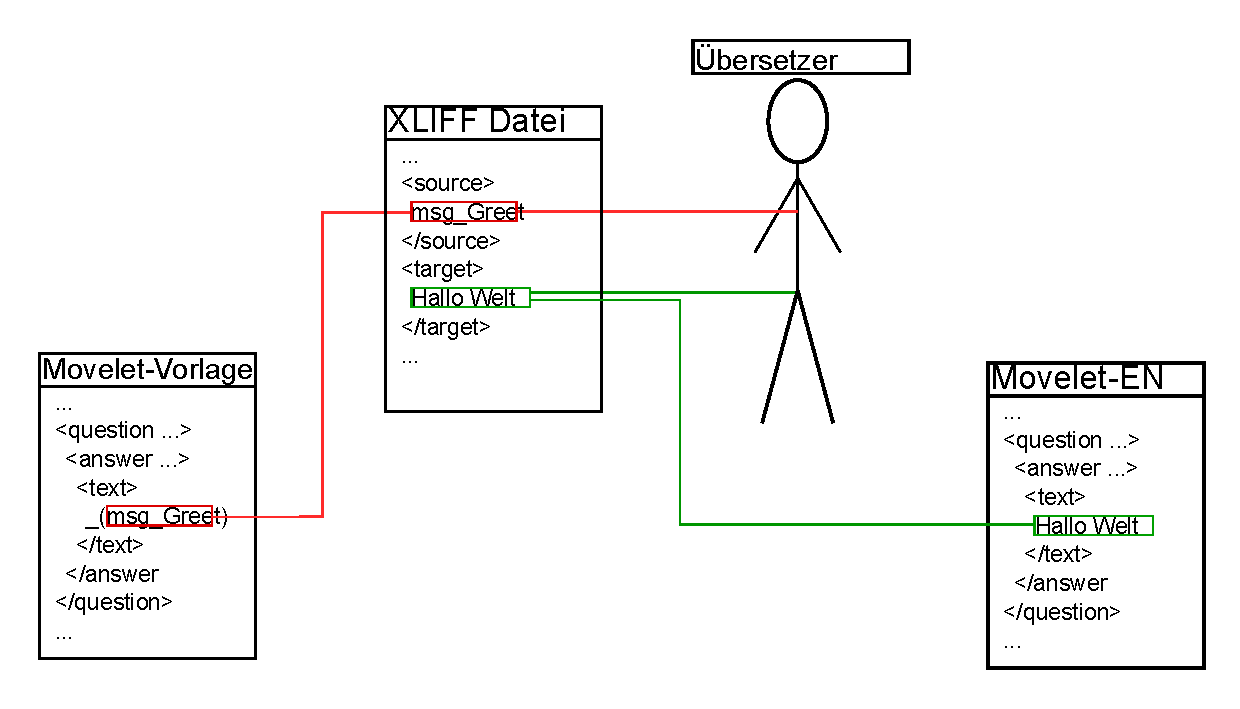
\includegraphics[width=1\textwidth]{img/zusammenfassung.pdf}
	\caption{Darstellung der Arbeitsschritte des Lokalisierungstools}
	\label{fig:zsm}
\end{figure}
\par
Das erarbeitete Lokalisierungstool greift bestehende Konzepte auf. Zu diesen Konzepten zählt die Auszeichnung von zu übersetzenden Strings, \ac{ITS}, \ac{XLIFF} und das Verwenden des Namens als Bezeichner. Die Auszeichnung von zu übersetzenden Strings, um diese von anderen Strings zu unterscheiden, wird von verschiedenen Lokalisierungstools verwendet. \ac{XLIFF} wurde von \ac{OASIS} für den Austausch von Daten der Lokalisierung entwickelt. Den Namen als Bezeichner zu verwenden ist ein grundlegendes Konzept der Bezeichnung.
\par
Das Alleinstellungsmerkmal des erarbeiteten Lokalisierungstools ist seine Einsatzmöglichkeit und Anpassung im Kontext von Movelets. Daher ist es die erste Software, die zum Zweck der Lokalisierung von Movelets eingesetzt werden kann. Aufgrund dessen hat dieses Lokalisierungstool das Potential den Prozess der Lokalisierung von Movelets zu revolutionieren.
\chapter{Diskussion}
Im Verlauf dieser Arbeit wurden die Anforderungen an das Lokalisierungstool anhand des Ziels dieser Arbeit formuliert. Für diese Anforderungen wurden Lösungsansätze anhand der Literatur recherchiert und diskutiert. Infolgedessen lassen sich Anforderungen und Lösungsansätze anhand der angegebenen Literatur nachvollziehen. Die Entscheidung für den jeweiligen Lösungsansatz wurde anhand einer Diskussion belegt.
\par
Ziel dieser Arbeit ist die Konzeption einer Software, welche zu übersetzende und übersetzte Strings der Texte eines Movelets automatisiert verarbeitet. Das erarbeitete Lokalisierungstool automatisiert die Extraktion ausgezeichneter Strings und das Ersetzen dieser durch deren Übersetzungen. Auf diese Weise wird ein hoher Grad der Automatisierung erzielt. Die Auszeichnung und Übersetzung der zu übersetzenden Strings erfolgt jedoch manuell und bietet folglich weitere Möglichkeit der Automatisierung. Resultierend daraus ist dieses Lokalisierungstool der Anfang einer Automatisierung der Lokalisierung von Movelets. Des Weiteren sind zum Zweck der Implementierung und Verwendung des Lokalisierungstools weitere Aspekte zu beachten. Diese sind die Konzeption der Benutzeroberfläche des Lokalisierungstools, die Auswahl der Übersetzer, beziehungsweise der Übersetzungssoftware und eine Dateistruktur für generierten \ac{XLIFF} Dateien. Zur Konzeption der Benutzeroberfläche zählt insbesondere das Auflisten und Behandeln von Kollisionen.
\par
Der Umfang dieser Arbeit ist aufgrund des von Movilizer vorgegebenen Zieles und dem vorgesehenen Umfang einer Projektarbeit begrenzt. Die Lokalisierung selbst jedoch umfasst weit mehr Aspekte. Zu diesen zählen.
\begin{itemize}
	\item Übersetzung
	\item Verwendung geeigneter Zeichensätze
	\item Übersetzung verknüpfter Strings
	\item Anpassung von Grafiken und Symbolen
	\item Anpassen der Benutzeroberfläche an Textlängen und Flussrichtungen
	\item Anpassung an geltendes Recht
	\item Anpassung der Formate für Adresse, Datum et cetera
	\item Anpassung der Maßeinheiten für Gewicht, Währung, et cetera
	\item Anpassung der Sortierung und Suche
\end{itemize}
In der Konsequenz bietet die Lokalisierung viel weiteres Automatisierungspotential für Movilizer. Bezogen auf dieses Lokalisierungstool selbst lassen sich weiter Forschungsaspekte empfehlen. Hierzu zählt die automatisierte Übersetzung der generierten \ac{XLIFF} Dateien. Anstelle von einer automatisierten Übersetzung bietet sich die Konzeption der Möglichkeit einer Übersetzung in der Benutzeroberfläche des Movelets selbst an. Dies ermöglicht die Verfügbarkeit alle Kontextinformationen bezüglich der Übersetzung. Des Weiteren ist es wissenswert, wie der Einsatz der in den \ac{XLIFF} Dateien gespeicherten Übersetzungen zum Aufbau einer Terminologiedatenbank oder eines \ac{TM} möglich ist, welche die Übersetzungskosten senken und die Übersetzungsqualität steigern.

%--------------------------------
% Start des Nachtexte der Arbeit
%--------------------------------
%	Literaturverzeichnis
\ihead{} % Neue Header-Definition
\printbibliography[title=Literaturverzeichnis]
\cleardoublepage

% Der Anhang beginnt hier - jedes Kapitel wird alphabetisch aufgezählt. (Anhang A, B usw.)
\appendix
\ihead{\appendixname~\thechapter} % Neue Header-Definition

% appendix.tex einziehen
\chapter{Anhang}

\section{Implementierung der Extraktion zu übersetzender Strings anhand einer Auszeichnung}
\label{sec:implementierung}
Zu dem Zweck der Implementierung eines Lokalisierungstools, welches die ausgezeichneten Strings extrahiert, ist für \ac{ITS} ein Namespace-based Validation Dispatching Language 
\autocite[Vgl.][]{ISO.2006}
Dokument gegeben.
\autocite[Vgl.][]{Filip.2013}
Die Auszeichnung \textit{\_()} lässt sich durch die Produktion einer kontextfreien Grammatik wie in \ref{eq:grammar} dargestellt definieren. Die dargestellte Produktion ist teil einer kontextfreie Grammatik, welche auch eine reguläre Grammatik ist, sie wird in der Augmented Backus"~Nauer Form 
\autocite[Vgl.][]{Crocker.2008} 
dargestellt.
\begin{align} \label{eq:grammar}
	\begin{array}{lcl}
		Q & = & \text{'''''} \text{ } | \text{ } \text{''''''} \\
		WS & = & (\epsilon \text{ } | \text{ } WSP \text{ } | \text{ } CR \text{ } |\text{ } LF)^* \\ 
		STRING & = & (VCHAR \text{ } | \text{ } DIGIT \text{ } |WS)^* \\
		MARKUP0 & = & \text{''\_(''} \text{ } WS \text{ } STRING \text{ } WS \text{ } \text{'')''} \\ 
		& & \text{; 0 steht für alle ohne ' ausgezeichneten Strings} \\
		MARKUP1 & = & \text{''\_(''} \text{ } WS \text{ } Q \text{ } STRING \text{ } Q \text{ } WS \text{ } \text{'')''} \\
		& & \text{; 1 steht für alle mit ' ausgezeichneten Strings} \\
		MARKUP2 & = & \text{''\_(''} \text{ } WS \text{ } \text{''concat(''}  \text{ } WS  \text{ } (CALL \text{ } \\
		& & \text{; 2 steht für alle concatinierten Strings} \\
		& | & \text{ } Q \text{ } STRING \text{ } Q ) \text{ } (WS  \text{ } \text{'',''} \text{ } WS \text{ } (CALL \text{ } \\
		& | & \text{ } Q \text{ } STRING \text{ } Q ) \text{ } )^+ \text{ } WS \text{ } \text{'')''} \text{ } WS  \text{ } \text{'')''} \\
		CALL & = & CHAR \text{ } STRING^* \\
		& & \text{ ; Aufruf von Variable oder Methode}
	\end{array}
\end{align}

% Ehrenwörtliche Erklärung ewerkl.tex einziehen
% !TEX root =  master.tex

\clearpage
\chapter*{Ehrenwörtliche Erklärung}

% Wird die folgende Zeile auskommentiert, erscheint die ehrenwörtliche
% Erklärung im Inhaltsverzeichnis.

% \addcontentsline{toc}{chapter}{Ehrenwörtliche Erklärung}
Ich versichere hiermit, dass ich die vorliegende Arbeit
 mit dem Thema: \textit{\DerTitelDerArbeit} selbstständig verfasst und keine anderen als die angegebenen Quellen und
Hilfsmittel benutzt habe. Ich versichere zudem,
dass die eingereichte elektronische Fassung mit der gedruckten Fassung übereinstimmt.

\vspace{3cm}
Ort, Datum \hfill \DerAutorDerArbeit



\end{document}
